\chapter{Screenshots}
\label{chap-captures}

Version~2 produces its own screenshots, with a fixed seed (option \code{-{}-screenshot}):
they always show the same game. The interface of the game is in French.

\begin{figure}[H]
    \centering
    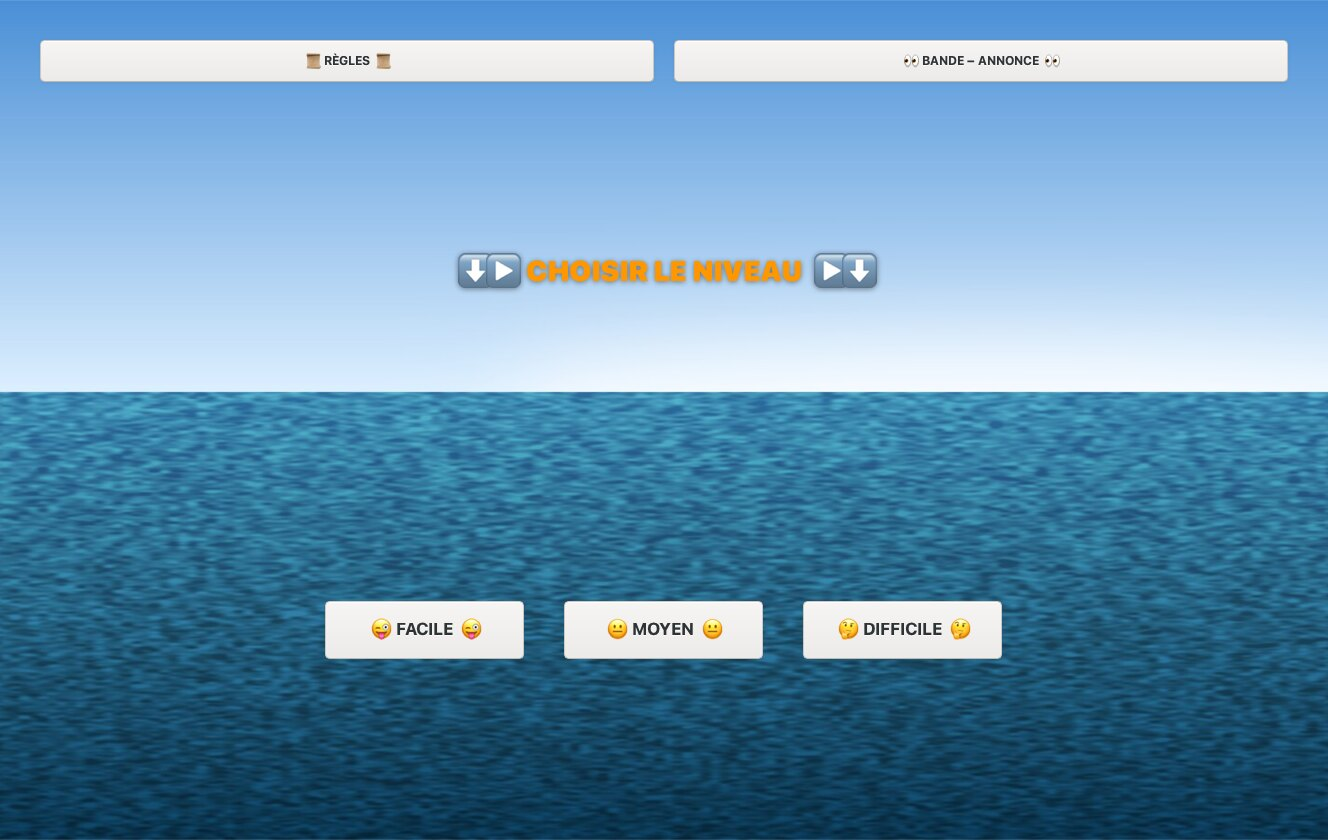
\includegraphics[width=0.78\textwidth]{../screenshots/menu.jpg}
    \caption{Version~2 --- choice of the level.}
\end{figure}

\begin{figure}[H]
    \centering
    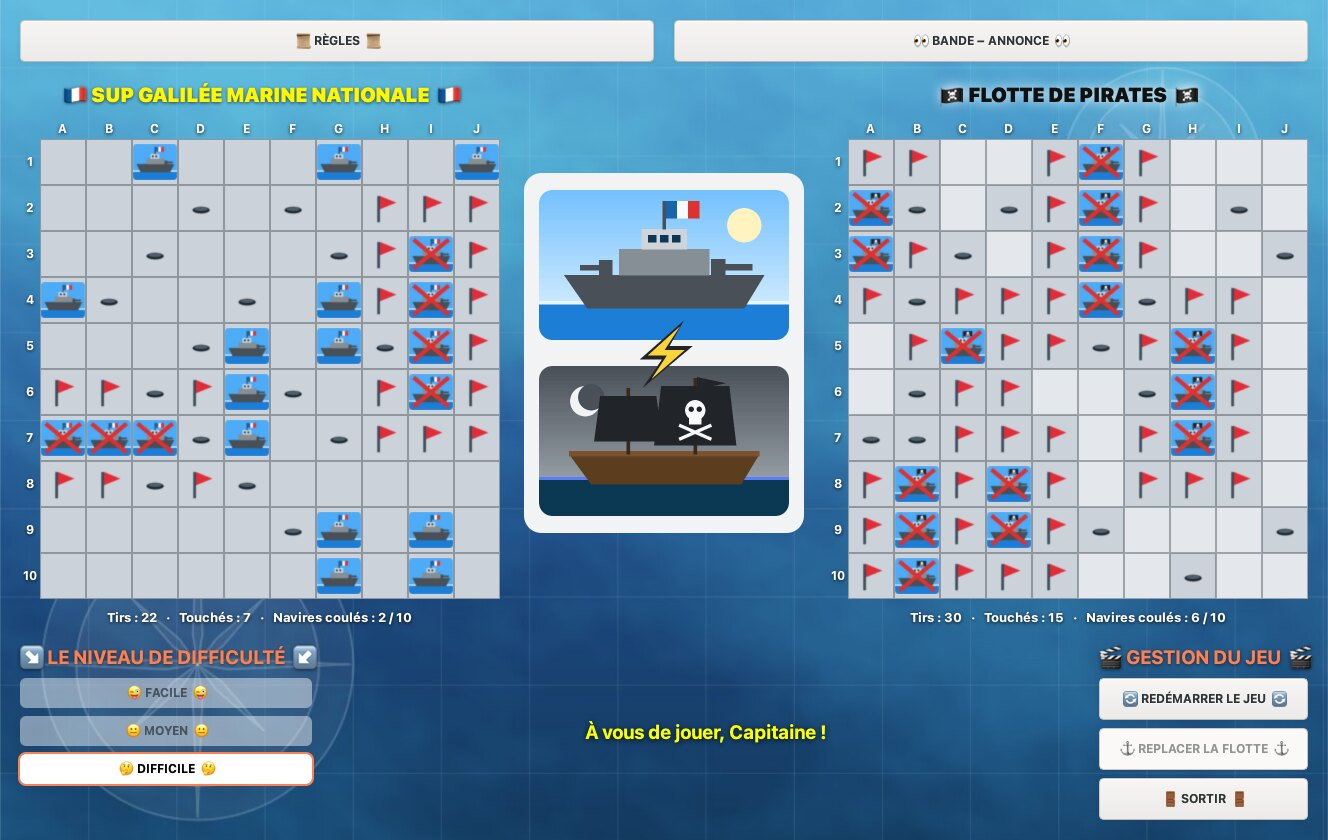
\includegraphics[width=\textwidth]{../screenshots/gameplay.jpg}
    \caption{Version~2 --- game in progress at the hard level. On the left, the flags show
        what the computer has deduced; on the right, what the player can deduce.}
\end{figure}

\begin{figure}[H]
    \centering
    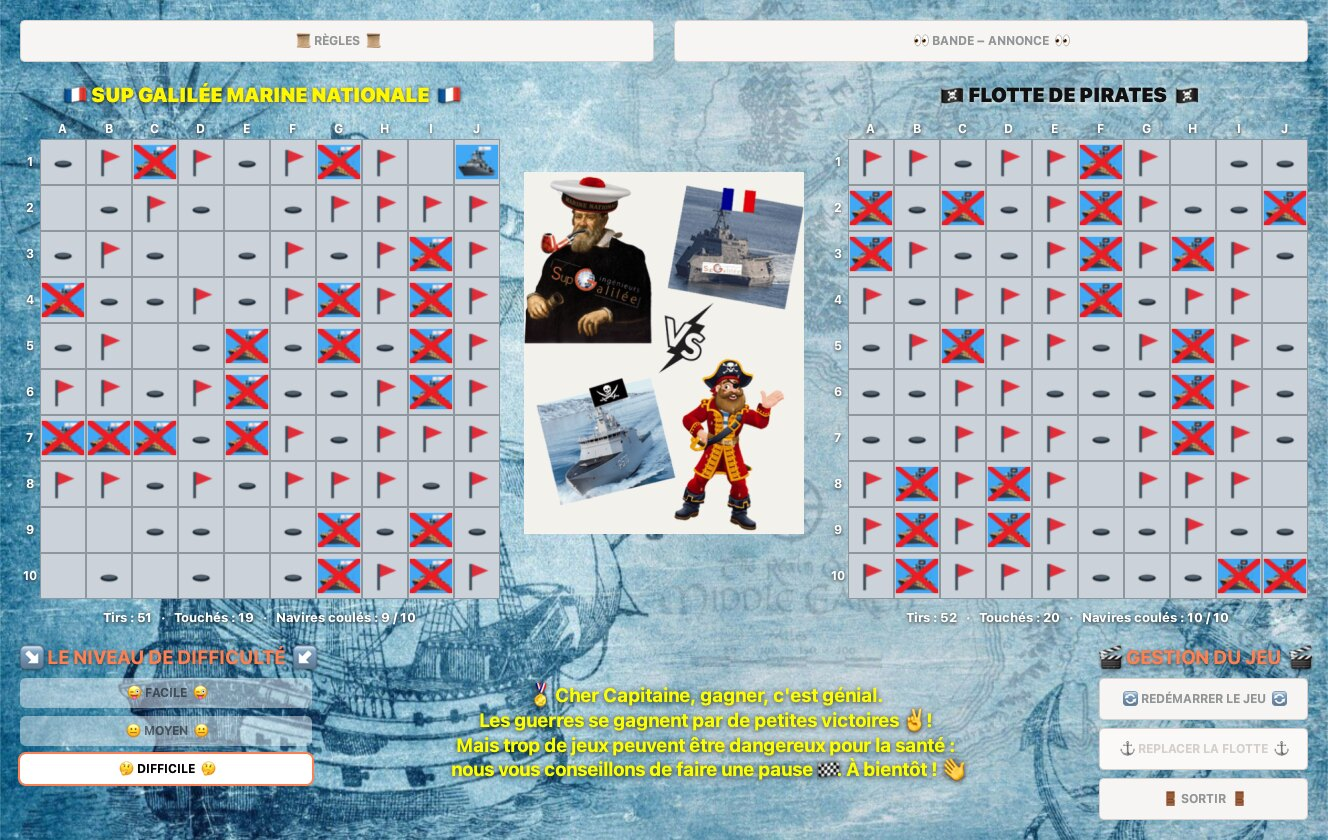
\includegraphics[width=\textwidth]{../screenshots/victory.jpg}
    \caption{Version~2 --- victory.}
\end{figure}

\begin{figure}[H]
    \centering
    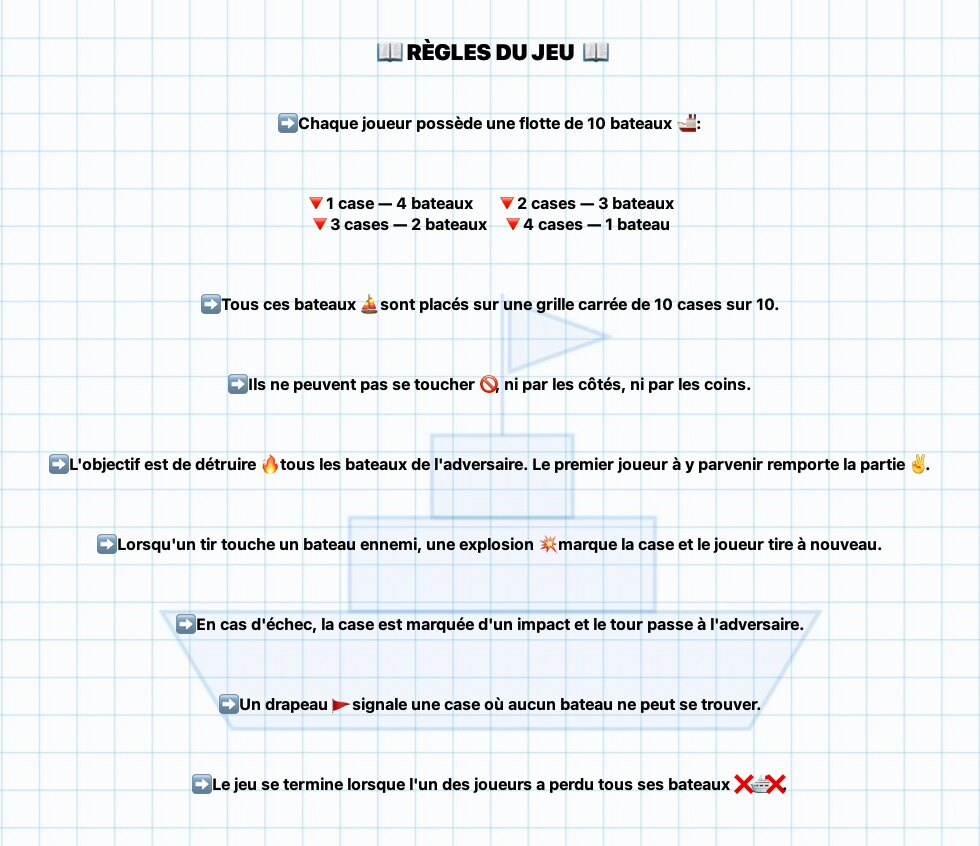
\includegraphics[width=0.8\textwidth]{../screenshots/rules.jpg}
    \caption{Version~2 --- rules window.}
\end{figure}

\begin{figure}[H]
    \centering
    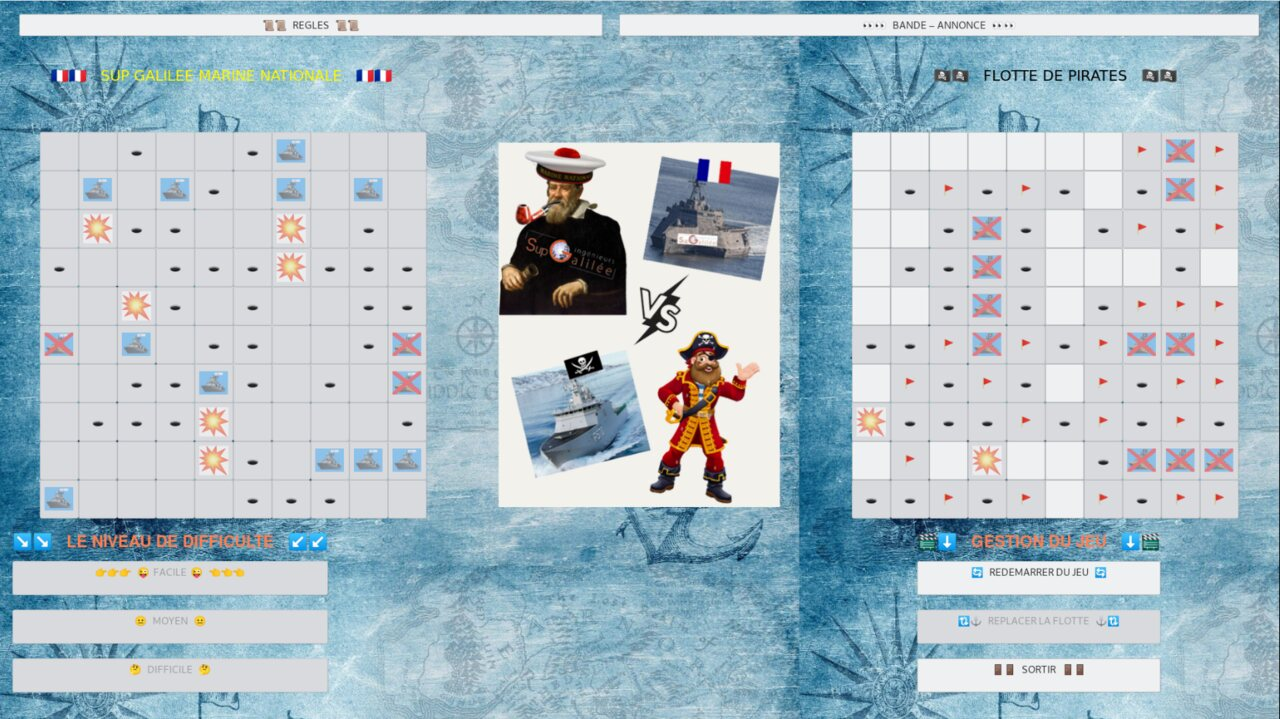
\includegraphics[width=\textwidth]{../screenshots/v1/gameplay.jpg}
    \caption{Version~1 (2023) --- game in progress. The visual identity has been kept.}
\end{figure}
